% This section provides the necessary context to help the reader understand the remainder of the thesis.

% Why this report is generated

In the section~\ref{sec: Intro}, its been highlighted how fraud can impact the business and overall economy. As per the PwC survey on crime and fraud~\caption{1} we can see that companies who invested money on fraud prevention had to pay 16\% less fine and\/ or penalties than who didn't~, as shown in figure~\ref{fig:fraud_preven}. Hence to protect financial and reputation losses, the companies have to invest money and effort. However the existing process is costly and human intensive. The paper focus on how a machine leaning based system can help the companies to reduce the overall operational cost and save financial losses.

The aim of this paper is to perform a data driven approach to extract relevant data to build machine learning classification model to detect specious company for a leading trade credit insurance provider. The trade credit insurance provides protection to the business (customer of the insurance company) in the event their buyers fail to pay for the products or services. Considering the raise of fraudulence business in recent past, the insurance provider has to monitor each buyers extensively before approving any insurance policy. Considering the number of number of policies are so high, a machine learning based recommended system was implemented for UK market to detect suspicious companies. Since the implementation of the system the solution saved around 1M pounds. Due to the success of the UK model, the organization decided to implement similar recommendation ending in other market.

\begin{figure}[htp]
    \centering
    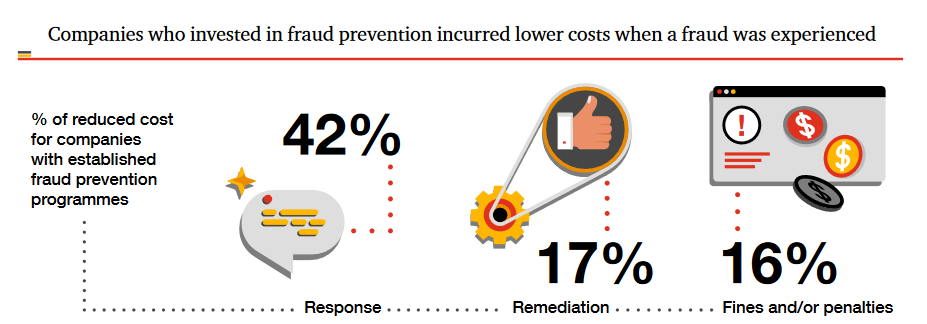
\includegraphics[width=\linewidth]{figures/prevent_fraud.PNG}
    \caption{Investment on Fraud Prevention. Source: PwC 2020 Fraud survey~\cite{PwC.Crime.Survey} }
    \label{fig:fraud_preven}
\end{figure}

For this paper, the a model focuses on identifying suspicious companies for Italian Market. Each country is fundamentally different in terms of trade credit policy. Hence, each country has its own internal process and method to identify the suspicious cases. To build the recommendation model below data driven machine learning strategies are used.

\mytodo{update terms: buyers, client and provider}

\subsection{Trade Credit Insurance}\label{subsec:trade-credit-insurance}
In business world trade credit is a regular practice done by manufactures, suppliers, and service providers to protect their financial interest from any types of risks.\mytodo{find the total yearly trade credit amount}. Companies sales their products and goods on credit to their buyers. Generally this is a continues process as back to back trade deals and payment happens between the suppliers and buyers. However, the amount of trade credit is very high, hence suppliers like to protect their interest by taking credit polices from financial institutions  \mytodo{cite what is trade credit}.

For financial institutions (credit insurance provider) ensures financial support to the supplier (client) in event of any mishaps. Trade credit is a risky business, hence before providing any insurance, financial institutions verifies both both supplier, sales, global economic conditions, external factors. As mentioned in section~\ref{sec: Intro}, due to the increased number of fraud cases, insurance providers have to also monitor fraudulent cases. Below are the types of fraud happens in the trade credit sector.

\begin{itemize}
    \item \textbf{Buyers Fraud:} When the buyers of the goods and products get benefited by not paying the dues to the suppliers.
    \item \textbf{Client Fraud:} When suppliers, the clients of the insurance company try to economic gain by doing insurance fraud.
    \item \textbf{Joint Fraud:} When the suppliers and buyers cooperate together to conduct insurance fraud get economic gain.
    \item \textbf{Internal Fraud:} When internal parties from the insurance company colludes with the client and conduct an insurance fraud.
\end{itemize}

In this study we will mainly focus on finding the suspicious buyers to prevent economic mishaps to protect the suppliers and the insurance companies from financial loss.


\subsection{Monitor Credit Policy}\label{subsec:monitor-credit-policy}

\subsubsection{Issuing Trade Insurance}\hspace*{\fill} \\
The trade insurance providers go through a sequence of steps to approve or issue a credit policy to their clients. In the the figure~\ref{fig:trade_credit}, the process of trade credit issuance is shown. First the client (supplier) requests for a credit policy to the trade credit insurance provider after they get a formal purchase request from their buyer. Based on the client's requests, the credit undertaking team of the insurance provider verifies the client, its buyer, the amount and other respective details of the transactions. If the credit undertaking team find the request as legitimate then they inform the internal operation team to issue a policy to the client. On a event the buyer fails to pay back for the goods, the supplier (client) applies for insurance claim from the service provider. After a thorough investigator the insurance provider pays the money to the supplier and tries to collect the money from the buyers to reduce its operational loss.

\begin{figure}[htp]
    \centering
    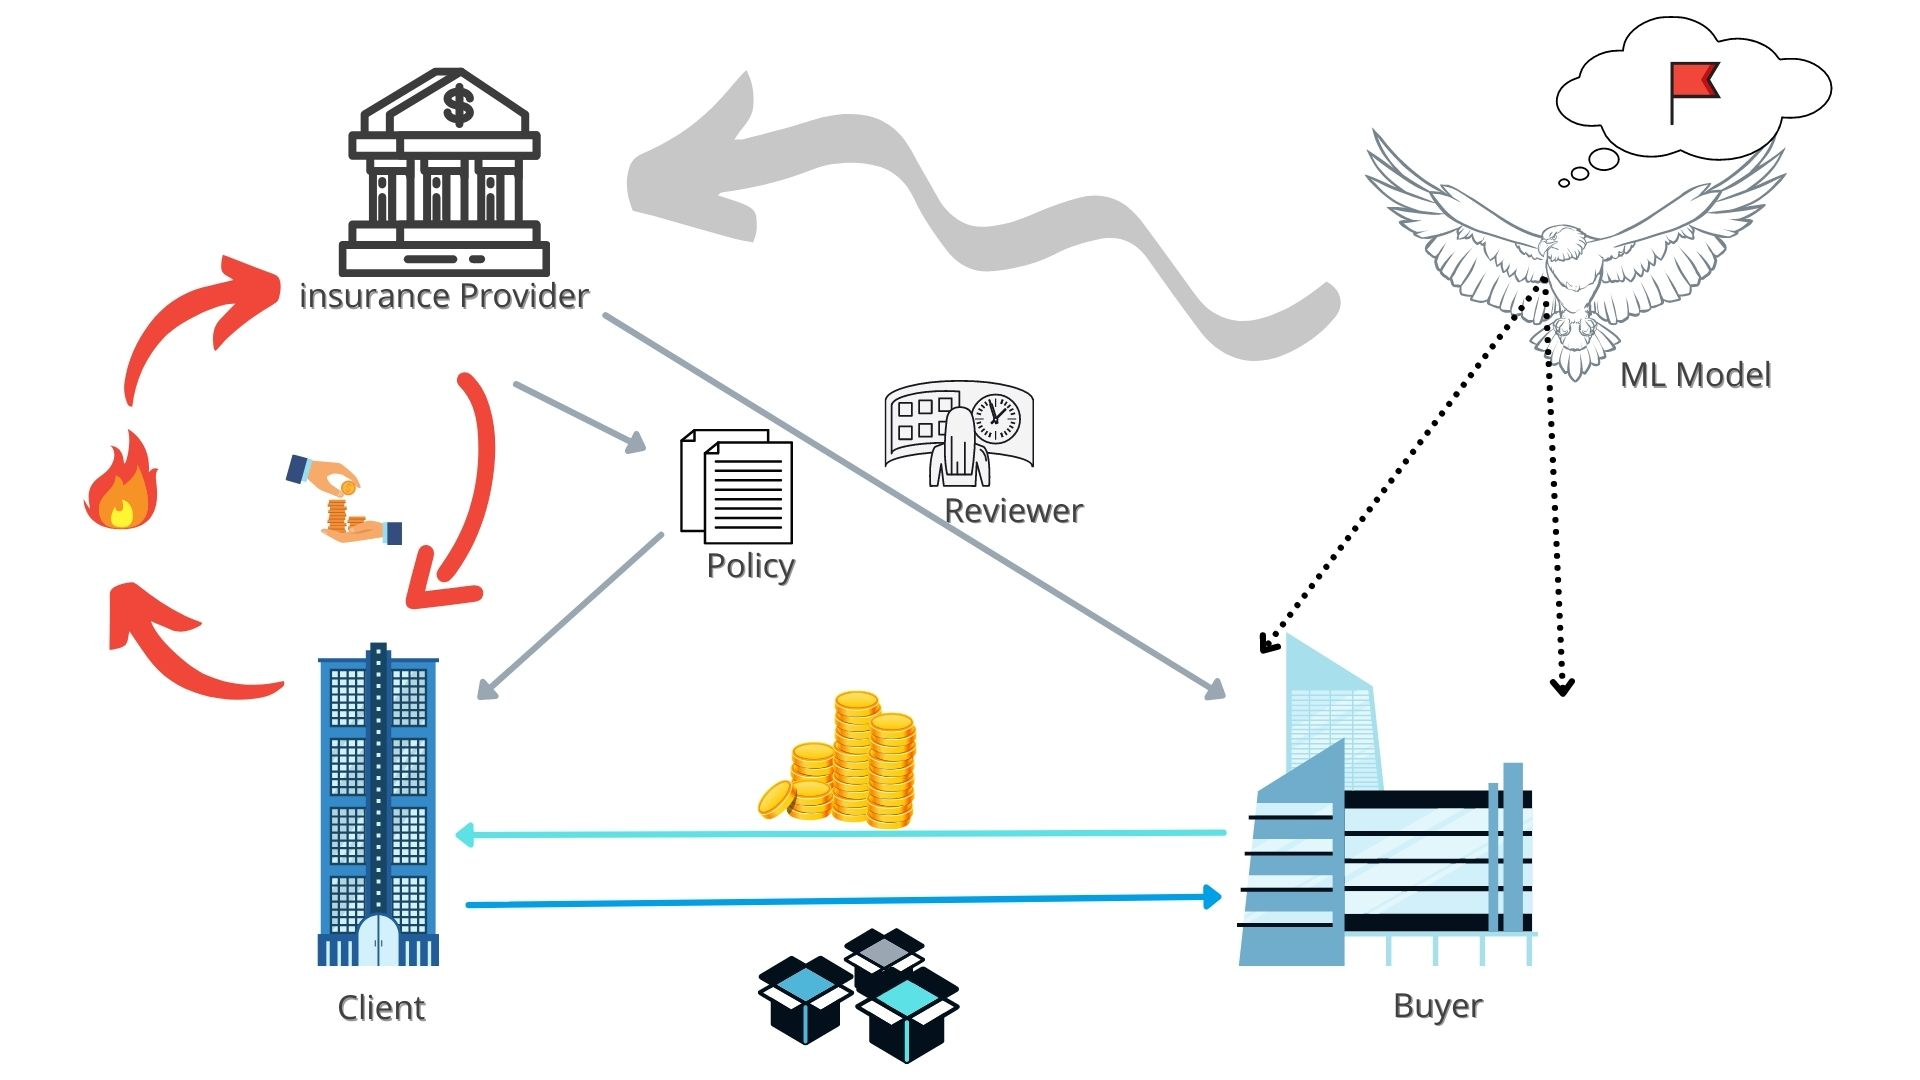
\includegraphics[width=\linewidth]{figures/monitor_buyers.jpg}
    \caption{Trade credit issuing process}
    \label{fig:trade_credit}
\end{figure}


As mentioned earlier in this chapter, there are four different types of fraud can take place in trade credit insurance sector. As the report only focuses on the buyers fraud, the existing monitoring process and proposed monitoring process are mentioned below to identify suspicious buyers.
\subsubsection{Traditional Approach}\hspace*{\fill} \\

The traditional way of identifying suspecious buyers are done by reviews from the credit undertaking team of the insurance service provider. As mentioend in Section~\ref{sec: Intro} below tools and techniques are currently use by the team.
\begin{itemize}
    \item{Internal System:} The reviews looks for suspecious patterns on the comapny reports and different system inicators to identify any suspecious companies.
    \item{External System:} The reviews also go through some external links provided by global ALM and regulatory systems to avoid any existing risks.
    \item{Overall Review:} Beside the above system, there are mutiple layes of monitoring done by different reviews to reduce operational errors.
\end{itemize}

\subsubsection{Machine learning base Approach}\hspace*{\fill} \\

In the proposed data-driven machine learning technique, a suitable model will be developed based on the data extracted from different system by taking input from the experts. Everyday the latest policy requests will be fed to the model so that it can predict the highly specious companies. The highlighted companies will be then shared with the credit undertaking team to expedite their reviewing / monitoring process. Based on the outcome and feedback of the reviewr, the model will be continuerly updated to improve its performance.



